\documentclass{article}

\usepackage{titling}
\usepackage{graphicx}
\usepackage{hyperref}

\pretitle{%
    \begin{center}
    \LARGE
        \bfseries
        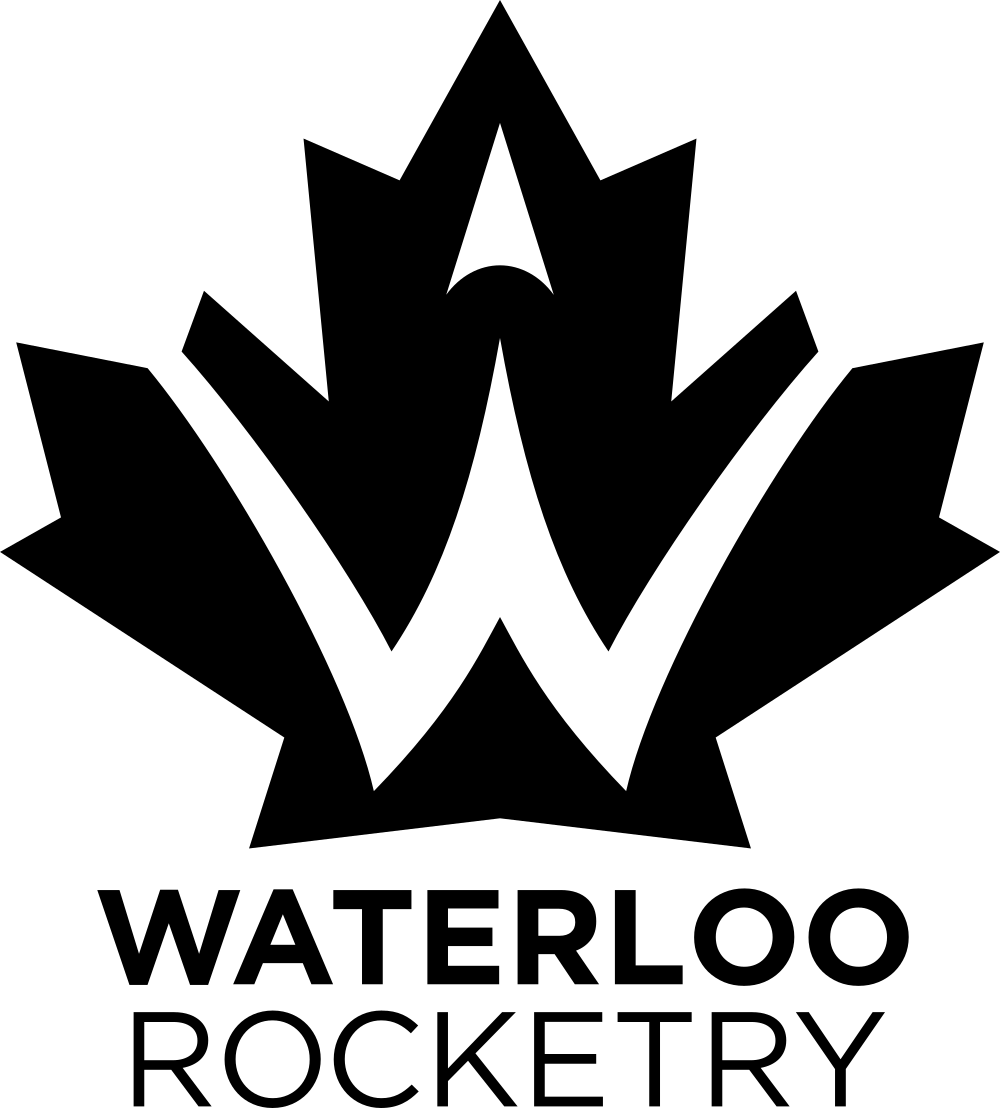
\includegraphics[width=6cm,height=6.6cm]{mono_standard}\\[\bigskipamount]
}
\title{Official Project Proposal - RLCSv2}
\posttitle{
    \end{center}
}

\author{Aaron Morrison}
\date{2017-08-02}

\begin{document}

    \pagenumbering{gobble}
    \maketitle
    \newpage
    \pagenumbering{arabic}

    \section{Background}
        RLCS is our Remote Launch Control System. It's purpose is to fill our rocket with nitrous oxide and then ignite the ignition spacer inside the rocket, all from a distance of 3000' away at launch control. To do so, it has control over 2 valves at the rocket (a valve for filling, and another valve for venting the fill lines), a linear actuator to disconnect the fill arm from the rocket, and 2 ignition coils inside the ignition spacer (all of these details are subject to change in future revisions of the rocket e.g. adding nitrogen super-pressurization would require more valves to load the nitrogen).It also features some basic data acquisition so we know how the fill is going (mass sensor underneath the rocket and a pressure transducer on the fill line)

        The first version of RLCS was built in early spring term of 2017, and came with us to IREC, and it worked, albeit with some undesirable limitations. The goal for the second version of RLCS (dubbed RLCSv2), is to remove these limitations and improve some other aspects of the system. For reference, I'm gonna make a list of all the problems with the first version.

        \begin{itemize}
            \item There was no actuator feedback from the tower side actuators to the users. We did not know if/when the valves turned, and the only indication that we had that ignition was working was that our rocket lifted off. To circumvent this, we had David stare at the rocket with binoculars and \emph{visually} (from 3000') confirm that stuff had happened.
            \item Different things were in different boxes. We had one box with the radio, and then ran CAT-5 cables from it to another box that controlled the ignition circuit, and another box that controlled the valves and disconnect actuator. This A), presented a tripping hazard what with all the cables going everywhere and B) introduced a source of headaches, because cables love breaking for no reason.
            \item There was no extensibility. If we wanted to add another valve, we would have needed to completely redesign one of the boxes, which would have taken a week or two.
            \item It didn't follow the Electrical Guidelines. It's a mission critical system, but it contained many components that we didn't have spares of. We had individual component spares, but since everything was soldered to veroboard, we couldn't actually swap them without a soldering iron.
            \item There wasn't any active cooling. One of the Lithium batteries got really hot because the desert's like 50 degrees. That's typically viewed as a not great thing to do.
            \item The display on the client side was awful. It was a 14x2 character LCD. It presented barely any information, and when LCD's get hot, they become unreadable.
            \item The antenna wasn't nearly powerful enough. We did not have client-tower contact at ground level, so the only reason it worked is because the judges let us up on their control tower 20 feet up. They may not let us do that next year, so let's go ahead and fix that.
            \item All data that was acquired (from the pressure transducer and the mass sensor) wasn't logged anywhere. It would have been nice to review that data later.
        \end{itemize}

    \section{Objectives}
        The primary goal for RLCSv2 is to fix all those problems above. The secondary goal is to fix all the new problems that come up while building the second version. Optimally, once v2 is done, we would not need to redesign any part of this system for at least 5 years. That means it needs to be robust as all hell and easily extensible to meet the future needs of our team.

    \section{The basic plan}
        The plan is to rebuild every piece of the system. For cleanliness, I plan to divide the work into three categories: Client Side, Tower Side, and Communications Link. The upgrades required in each category is as follows:
        \begin{enumerate}
            \item Client Side:
            \begin{itemize}
                \item Better display: this may either mean a bigger LCD to get more information on, or a full blown graphical display. Advantage to the LCD is that it can be driven by an Arduino (the monitor would need to be hooked to an raspberry pi or something), while the advantage of the monitor would be the more user friendly interface. Since the plan is to add way more sensors to the system this year, there will be more data to present to the user, so this is critical.
                \item More robust box: Preferably one where the buttons/switches are hidden underneath a lid or something (to prevent ingress of desert dust). This thing gets handled by humans, it should be able to withstand gentle shaking without falling to pieces.
                \item Data logging: put an SD card writer into the box. Make it record every reading that comes back from the tower side. There will also be data logging on the tower side, but data redundancy protects us from random screw-ups, like the tower side box catching on fire.
            \end{itemize}
            \item Tower Side (this is where most need to happen):
            \begin{itemize}
                \item Put everything in one (ridiculously robust) box: This would mean there are fewer weak cables that can break easily, and it would look much nicer.
                \item Put everything on modular PCBs: Veroboard is sketchy, I'd be much happier if everything was mounted on PCBs that can be easily swapped in and out. The advantage to modular PCBs is that if 1 component breaks, you replace 1 of many small PCBs instead of one massive one. Also, modularity implies better extensibility. If every valve/actuator has its own modular board, adding another valve just means adding another little board.
                \item Active cooling: Lithium Polymer batteries have this fun tendency to explode if they get too hot. The plan is to add a couple of 12 volt PC fans to the box, one to bring cool air in, and one to eject hot air.
                \item Sensors on everything: The biggest problem with v1 was no active feedback, we should aim to way overcompensate on this front. This means that every valve should have limit switches, every current carrying wire should have a current sensor on it. All this data should be logged (SD card probably), and reported back to the user.
            \end{itemize}
            \item Communication:
            \begin{itemize}
                \item We need to raise our antennas higher. I don't know much about radio, but antennas like to be high off the ground. Optimally we'd build a tripod for the client side antenna and mount our tower side antenna to the launch tower.
                \item Research: Like I said, I know almost nothing about radio. Before committing to any plans, there's a lot of reading that needs to be done. A good starting place is here \url{http://www.rohde-schwarz-usa.com/rs/rohdeschwarz/images/8GE01_Antenna_Basics.pdf}.
                \item The transceivers (XBee 900MHz modules) probably won't change. It would be cool to become ham certified and build our own high power transceivers (this would eliminate any chance of poor reception. Our current transceivers are like 1/2 watt, with ham certs we can build transceivers up to 1000 watt), this is likely beyond the range of possibility for this year.
            \end{itemize}
        \end{enumerate}

    \section{Obstacles}
        This is less of an Obstacles section than just a ``Things we should look out for'' section. I don't really know what to put here, so I'm just gonna make a list of things that we should bear in mind while working on this project.
        \begin{itemize}
        \item Keep good communication with other projects to remain aware of changing requirements

            After winning at IREC, we now have a list of several dozen projects that we'd like to work on before the 2018 IREC. Many of these projects will require changes to be made to RLCS. The planned design is extensible enough that adding stuff shouldn't be a problem, but it may still take some amount of time to do, so being aware of any changes that need to be made as soon as possible would be very helpful.
        \item Involve new people

            There's enough work to be done on this project that we could absolutely have some frosh working on it. There's research to be done, UIs to be designed, stuff to be soldered, boxes to be laid out, laser cuttings to be drawn and done, cables to be managed, documentation to be written, and testing to be carried out. Most of this work isn't that hard, so it'd be easy to integrate first years if any of them are interested in getting into this stuff. It'd also be great to get more full members familiar with this system in case I'm not at competition next year (I'm on coop).
        \end{itemize}

    \section{Testing Required}
        We need to unit test the software, test the system in flight configuration, and stress test the boxes under heat to see how long they last. We also need to perform new range tests on the communication system to make sure that it will exceed the range that we need it to work at for competition. For 2017, this project was so rushed that most of this testing never got done, since we have time, we should test this system to failure.

    \section{Cost Breakdown}
        Again, by section
        \subsection{Tower Side}
            \begin{itemize}
                \item Box: Optimally we'd get this sponsored (I'm planning to email Pelican and plasticase (they make Nanuk boxes)), but barring that, this toolbox (\url{http://www.dewalt.ca/en-ca/products/gear-and-equipment/tool-storage/toughsystem-ds130/dwst08130}) would probably work great for \$50.
                \item PCBs: Each actuator (there are currently 4) needs a modular PCB, the boards themselves are cheap as hell, the required components cost \$15 per board. Counting spares, this works out to about \$100 all told.
                \item Power: We have LiPo batteries, but the circuitry for stepping voltages and distributing power will probably cost about \$30.
                \item Arduino: With all the sensors, we'll need to run off of an Arduino Mega. These cost \$50.
                \item Cabling: Inside the box, about \$20. Connectors, however, get expensive. Glenair is apparently interested in a sponsorship, and I plan to reach out to Amphenol as well, but without sponsorship, kick ass connectors would be about \$100, and actuator cables will probably cost \$50.
            \end{itemize}
            All told, without sponsorship, \$400.

        \subsection{Client Side}
            \begin{itemize}
                \item Box: Same as tower side. It can probably be sponsored, but if not it'll be about \$50.
                \item Switches: We could steal them from v1, but sparkfun sells missile switches for \$3. All the switches can be bought for \$30.
                \item Arduino: I'd like to have another Mega, since it will mean we only need one spare, instead of a spare for the tower side and another for the client side. So another \$50.
                \item Data logging: \$30 for SD card writers here and on the tower.
            \end{itemize}
            All told, without sponsorship: \$160.

        \subsection{Communication}
            I don't know. If we just need to mount to the launch tower and build a client side tripod tower thing out of PVC piping, it can be done for \$50 plus the cost of coax cables (maybe another \$50). If we want new antennas (research is required), it will be more expensive.

\vspace{2cm}

        The best guess that I can make for cost, using the above numbers, is \$600-700 without sponsorship, getting boxes and connectors sponsored would drop that to \$400-500. Everything always goes over budget, but securing another \$600 in cash and boxes/connectors would probably be safe (Robin reports that we already have \$200 from WEEF).

\end{document}
